\documentclass[UTF8,zihao=-4]{ctexart}
\usepackage[a4paper,margin=2.5cm]{geometry}
\usepackage{amsmath, amssymb, amsthm}
\usepackage{bm}
\usepackage{hyperref}
\usepackage{graphicx}
\usepackage{caption}
\usepackage{listings}
\usepackage{xcolor}
\usepackage{float}
\usepackage{booktabs}
\usepackage{longtable}
\usepackage{multirow}
\usepackage{placeins}
\graphicspath{{figures/}}

% 代码样式
\lstdefinestyle{code}{
  basicstyle=\ttfamily\small,
  numbers=left,
  numberstyle=\tiny,
  numbersep=8pt,
  keywordstyle=\color{blue},
  commentstyle=\color{teal!70!black},
  stringstyle=\color{orange!70!black},
  showstringspaces=false,
  breaklines=true,
  frame=single,
  framerule=0.3pt,
  rulecolor=\color{black!15}
}
\lstset{style=code}

\title{Prompt 工程实践:从零样本到自动化优化}
\author{}
\date{\today}

\begin{document}
\maketitle

\section{Zero-shot, Few-shot, Chain-of-Thought}
\subsection{三种模式的演进范式}
零样本(Zero-shot)依赖模型预训练语义先验,在没有显式示例时直接完成任务;少样本(Few-shot)通过提示语中的示例建立任务上下文;Chain-of-Thought(CoT)进一步鼓励模型显式拆解思路。图\ref{fig:prompt_modes_cn} 展示了这三种模式从简单指令到结构化推理的渐进关系。
\begin{figure}[H]
  \centering
  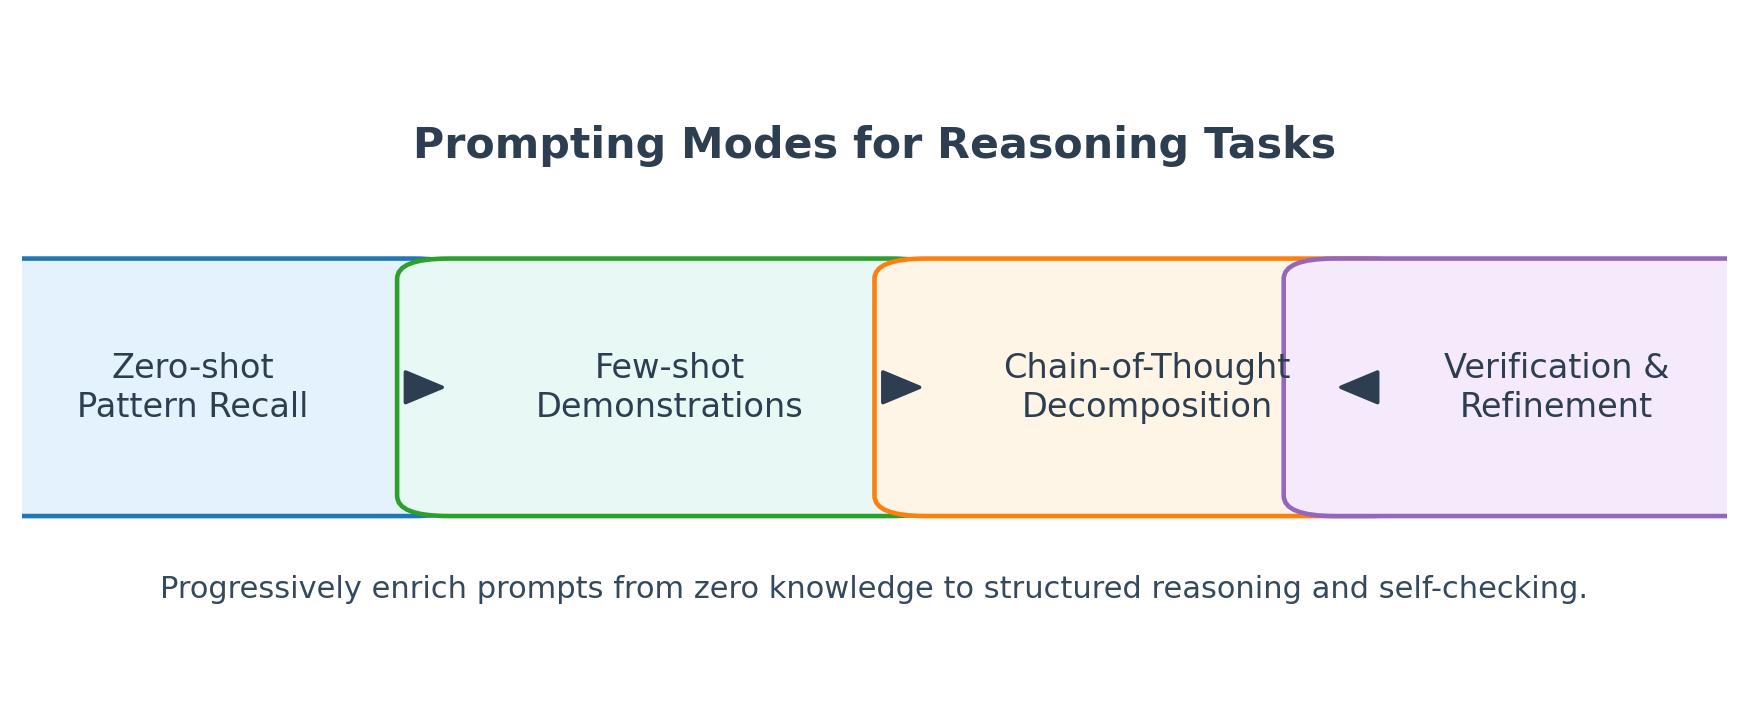
\includegraphics[width=0.92\textwidth]{prompt_modes.png}
  \caption{Prompt 模式演进:从零样本到少样本,再到 Chain-of-Thought 与结果验证。}
  \label{fig:prompt_modes_cn}
\end{figure}

\subsection{零样本策略}
\begin{itemize}
  \item \textbf{指令明确化:} 明确任务、输出格式、风格,例如“用中文总结以下段落并列出关键要点”。
  \item \textbf{约束与角色:} 通过系统提示(system prompt)设定模型角色,如“你是一个法律顾问”。
  \item \textbf{语义锚点:} 包含关键词、上下文背景(领域、时间范围)以减少歧义。
\end{itemize}
零样本适合知识问答、简单分类等任务,但在推理或多步工作流上可靠性有限。

\subsection{少样本构造原则}
\begin{itemize}
  \item \textbf{示例多样性:} 覆盖不同类别、边界情况,避免模型过拟合单一示例。
  \item \textbf{输入输出对齐:} 使用一致的格式(JSON、Markdown 列表)并强调所需字段。
  \item \textbf{位置敏感性:} 在开头放置最重要的示例,确保模型优先关注。
  \item \textbf{错误示例:} 在复杂任务中给出错误案例及修正示范,提高模型自检能力。
\end{itemize}

\subsection{Chain-of-Thought 提示}
CoT 通过“让我们逐步思考”类提示引导模型输出中间推理步骤,常见技巧:
\begin{itemize}
  \item \textbf{解释模板:} 使用“问题→分析→答案”结构,引导模型生成分步解答。
  \item \textbf{算术、逻辑任务:} 将复杂问题拆分为子问题,如设未知数、列方程、做单位换算。
  \item \textbf{外部验证:} 联合 self-consistency(多次采样取众数)或 verifier 模型,降低随机性。
\end{itemize}
在部署中,可结合 Temperature=0(确定性)与 Beam Search 等策略平衡稳定性与覆盖度。

\section{ReAct(Reason + Act)与 Tree-of-Thoughts}
\subsection{ReAct 工作流}
ReAct 将思考(Reason)与行动(Act)交替进行:先生成下一步推理,再调用工具或执行查询,然后基于结果继续推理。典型应用包括开放领域问答、代码调试、数据检索。基本流程:
\begin{enumerate}
  \item 设定环境:描述可用工具(搜索、计算、数据库查询)及调用方式;
  \item Prompt 模板:`Thought: ...`,`Action: tool_name[input]`,`Observation: ...`;
  \item 迭代执行直到达到 `Final Answer:`。
\end{enumerate}
实现时需限制循环次数、过滤重复动作,并通过惩罚机制减少多余查询。

\subsection{Tree-of-Thoughts 框架}
Tree-of-Thoughts(ToT)将推理扩展为树状搜索,节点表示思路片段(thought),边表示状态转移。 \textbf{核心要素}:
\begin{itemize}
  \item \textbf{生成策略:} 在每一层生成多个候选思路,可使用 Beam Search、DFS/BFS 或蒙特卡洛树搜索(MCTS)。
  \item \textbf{评估函数:} 使用评分器(模型自身或外部 evaluator)评估节点质量,保留高分分支。
  \item \textbf{剪枝机制:} 对低分分支进行裁剪,控制 token 消耗。
\end{itemize}
ToT 适用于数学推理、规划任务、代码修复等需要探索多条路径的场景。需要注意树的扩展速度与 token 限制之间的平衡。

\subsection{综合架构示意}
图\ref{fig:reasoning_stack_cn} 展示了系统提示、状态记忆、ReAct 循环、ToT 搜索与工具/评估器的协同方式。
\begin{figure}[H]
  \centering
  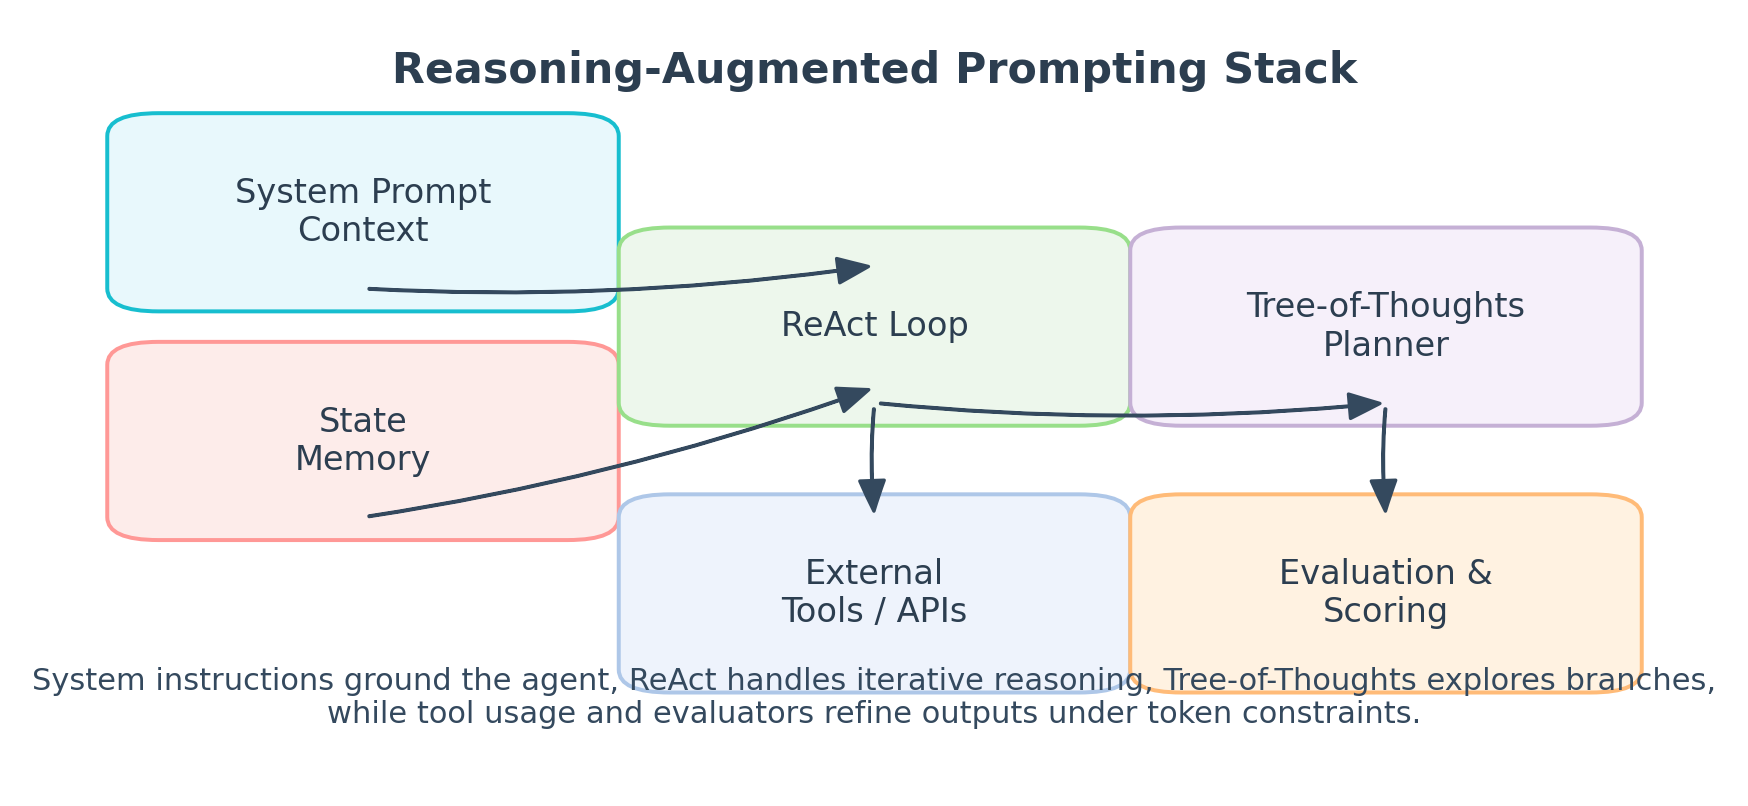
\includegraphics[width=0.92\textwidth]{reasoning_stacks.png}
  \caption{推理增强 Prompt 堆栈:System Prompt 约束行为,ReAct 处理交互式步骤,Tree-of-Thoughts 负责全局探索。}
  \label{fig:reasoning_stack_cn}
\end{figure}

\section{System Prompt、上下文窗口与 Token 限制}
\subsection{System Prompt 设计}
System Prompt 定义模型的角色、语气、遵守的准则,影响所有后续对话。设计要点:
\begin{itemize}
  \item \textbf{角色设定:} 描述专业背景(如“资深数据科学家”)、能力范围、应避免的行为。
  \item \textbf{输出规范:} 指定语言、格式、禁用词、保密要求。
  \item \textbf{安全策略:} 包含安全提示和拒绝策略,避免敏感内容。
\end{itemize}
复杂系统中可组合多段 System Prompt,并通过“安全头→专业头→任务头”的方式递进约束。

\subsection{上下文窗口管理}
上下文窗口(Context Window)决定单次对话可处理的最大 token 数。常见策略:
\begin{itemize}
  \item \textbf{分段与摘要:} 将历史对话压缩为摘要、要点或检索型记忆,仅保留关键信息。
  \item \textbf{检索增强:} 结合向量数据库实现“按需注入”上下文,而非始终保存全部历史。
  \item \textbf{窗口滑动:} 对低优先级历史内容进行裁剪,将 token 留给最新信息。
  \item \textbf{结构化消息:} 使用 JSON/Markdown 等统一格式,便于自动裁剪与解析。
\end{itemize}

\subsection{Token 预算与估算}
控制 token 消耗可提升稳定性与成本效率。建议:
\begin{itemize}
  \item \textbf{预算表:} 为系统提示、用户输入、参考资料、模型输出分别设定 token 上限。
  \item \textbf{估算工具:} 使用 `tiktoken`、`transformers` 的 tokenizer 提前计算,或在服务端统计每次请求的实际消耗。
  \item \textbf{降级策略:} 在超过阈值时自动触发摘要、删除低权重消息或换用短格式。
\end{itemize}
\begin{longtable}{p{3cm}p{3cm}p{4cm}p{4cm}}
\toprule
组成 & 典型长度 & 优化方法 & 风险 \\
\midrule
System Prompt & 200--600 token & 模块化分段、复用模板 & 过长导致主内容挤压 \\
Few-shot 示例 & 每个 50--200 token & 选择代表性案例、压缩输出 & 示例过多导致上下文溢出 \\
检索文档 & 200--2000 token & Top-$k$ 筛选、摘要压缩 & 噪声文档干扰模型 \\
模型输出 & 100--800 token & 指定最大长度、结构化模板 & 输出截断或跑题 \\
\bottomrule
\end{longtable}

\section{Prompt 优化与自动生成}
\subsection{手动优化流程}
\begin{enumerate}
  \item \textbf{明确目标:} 定义评估指标(准确率、拒绝率、用户评分)。
  \item \textbf{建立基线:} 收集典型输入与期望输出,形成评测集合。
  \item \textbf{迭代调整:} 使用差异测试(A/B)对比不同 prompt,在小批量上快速验证。
  \item \textbf{记录版本:} 使用 Git、实验追踪工具保存 prompt 模板、评测结果、迭代原因。
\end{enumerate}

\subsection{自动化优化技术}
\begin{itemize}
  \item \textbf{Prompt Tuning / Prefix Tuning:} 将 prompt 嵌入向量化,通过梯度更新优化虚拟 token。
  \item \textbf{黑盒优化:} 使用 Genetic Algorithm、Bayesian Optimization、Reinforcement Learning 搜索离散 prompt 空间。
  \item \textbf{Self-Refinement:} 让模型对自身输出评分并给出改进建议,再自动生成新 prompt。
  \item \textbf{Prompt Compression:} 通过 Distillation、LASSO、句子选择将冗长提示压缩至相同效果。
\end{itemize}

\subsection{自动生成示例}
\begin{lstlisting}[language=Python,caption={使用自反思自动生成新 Prompt}]
import json
from transformers import AutoModelForSeq2SeqLM, AutoTokenizer

model_name = "google/flan-t5-xxl"
tokenizer = AutoTokenizer.from_pretrained(model_name)
model = AutoModelForSeq2SeqLM.from_pretrained(model_name, device_map="auto")

seed_prompt = """
You are an AI writing assistant. Rewrite the paragraph in a more persuasive tone.
"""

feedback_template = """
Original prompt:
{prompt}

Task feedback:
1. Is the instruction specific and scoped?
2. Does it define output format?
3. Suggest improvements.
"""

inputs = tokenizer(feedback_template.format(prompt=seed_prompt), return_tensors="pt").to(model.device)
outputs = model.generate(**inputs, max_new_tokens=256)
analysis = tokenizer.decode(outputs[0], skip_special_tokens=True)

refinement_template = """
Given the original prompt and the feedback, produce an improved prompt.
Original prompt: {prompt}
Feedback: {feedback}
"""

inputs = tokenizer(refinement_template.format(prompt=seed_prompt, feedback=analysis), return_tensors="pt").to(model.device)
outputs = model.generate(**inputs, max_new_tokens=128)
improved_prompt = tokenizer.decode(outputs[0], skip_special_tokens=True)

print(json.dumps({"improved_prompt": improved_prompt, "feedback": analysis}, indent=2, ensure_ascii=False))
\end{lstlisting}
此流程通过 LLM 自我审阅和再生成实现 prompt 自动改写,可结合外部评测或人类标注进一步筛选。

\section*{实践建议}
\begin{itemize}
  \item 为不同业务场景维护 Prompt 库与复用模板,统一命名与版本控制。
  \item 构建离线评测集及在线指标,确保 Prompt 修改对业务影响可量化。
  \item 在长上下文场景结合检索与摘要策略,避免系统提示与示例挤占窗口。
  \item 对自动生成的 Prompt 进行人工审查,避免出现偏见、安全合规问题。
\end{itemize}

\section*{参考文献}
\begin{itemize}
  \item Wei et al. ``Chain-of-Thought Prompting Elicits Reasoning in Large Language Models.'' NeurIPS, 2022.
  \item Yao et al. ``ReAct: Synergizing Reasoning and Acting in Language Models.'' ICLR, 2023.
  \item Yao et al. ``Tree of Thoughts: Deliberate Problem Solving with Large Language Models.'' arXiv, 2023.
  \item Zhou et al. ``Large Language Models Are Human-Level Prompt Engineers.'' arXiv, 2022.
  \item Kojima et al. ``Large Language Models are Zero-Shot Reasoners.'' NeurIPS, 2022.
\end{itemize}

\end{document}

